\chapter{Introduction} % (fold)
\label{cha:Introduction}


\begin{abstract}
This chapter places this dissertation in the context of
modern societies and its challenges. Specifically, we
motivate this thesis by the demographic changes in the
global North. In the following, we recall past approaches to
trajectory generation and discuss their limitations.
Finally, we present the contributions and the outline of
this dissertation.
\end{abstract}

\newpage


\section{Robots under the eyes of demographic change}

In a world struggling with the challenges of an aging
population, shifting demographics, and a scarcity of
affordable labor for physically demanding tasks, the need
for technological solutions is more pronounced than ever
\cite{ince2015economic}.
Technological progress in the corresponding field of
robotics today is disappointing, especially in an era where
the non-embodied counterpart is touching all of our lives.
While strides in natural language processing and computer
vision have significantly improved our office activities,
embodied systems still lag behind in sophistication and core
capabilities.

\begin{figure}[h]
  \begin{subfigure}{0.5\textwidth}
    \centering
    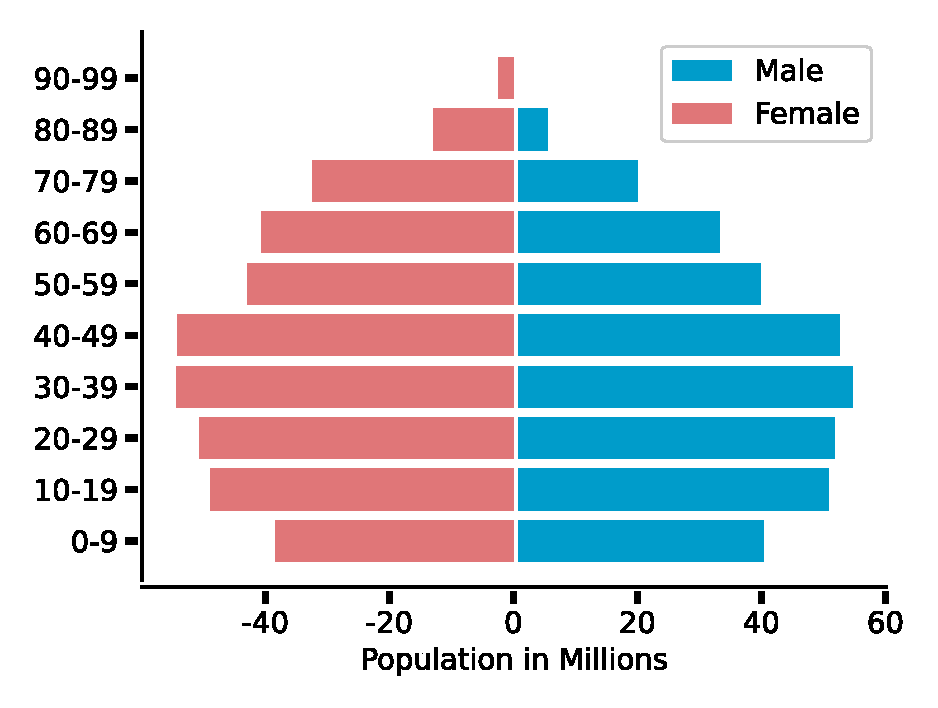
\includegraphics[width=0.9\textwidth]{src/introduction/img/population_2000.eps}
  \end{subfigure}%
  \begin{subfigure}{0.5\textwidth}
    \centering
    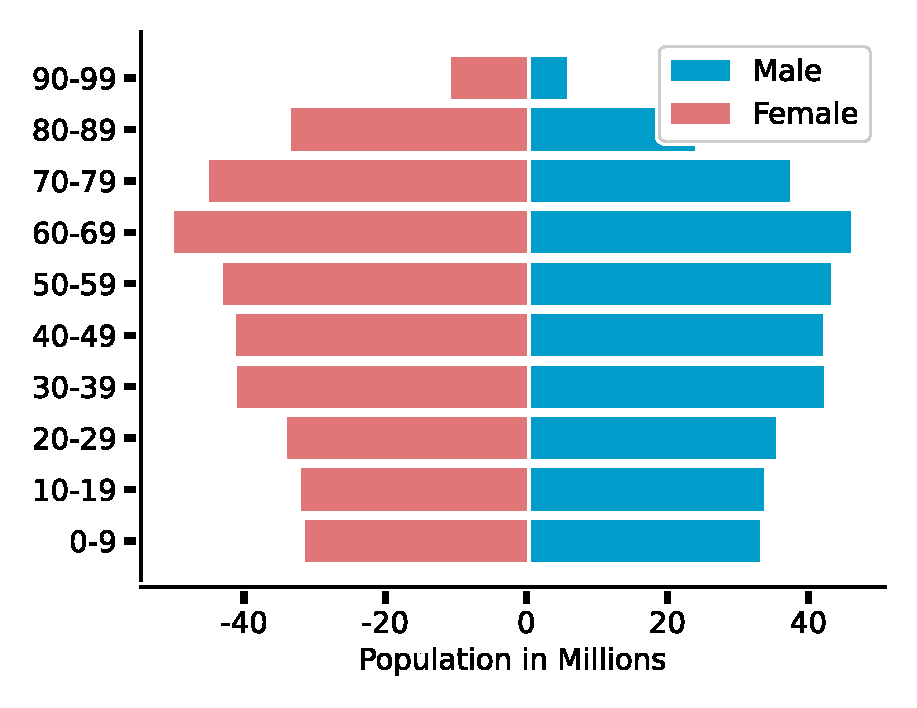
\includegraphics[width=0.9\textwidth]{src/introduction/img/population_2050.eps}
  \end{subfigure}
  \caption
  []
  {
    Population portions by age in 2000 (left) and predictions for
    2050 (right) in Europe. The aging society leads to labor shortage
    which may be counterbalanced with increase in
    automation. \footnotemark
  }
\end{figure}

\footnotetext{
    United Nations, Department of
    Economic and Social Affairs, Population Division (2022)
}

Industrial robots, see \cref{fig:industrial_robot}
are highly capable in certain tasks, but
often lack the nuanced understanding and safety required for
dynamic, human-shared environments. Collaborative robots
provide more safety capabilities through a lightweight
hardware design and sensors, see
\cref{fig:collaborative_robot}. These
robots are designed to exist safely alongside their human
counterparts using different low-level control appraches.

\begin{figure}
  \centering
  \begin{subfigure}{0.5\textwidth}
    \centering
    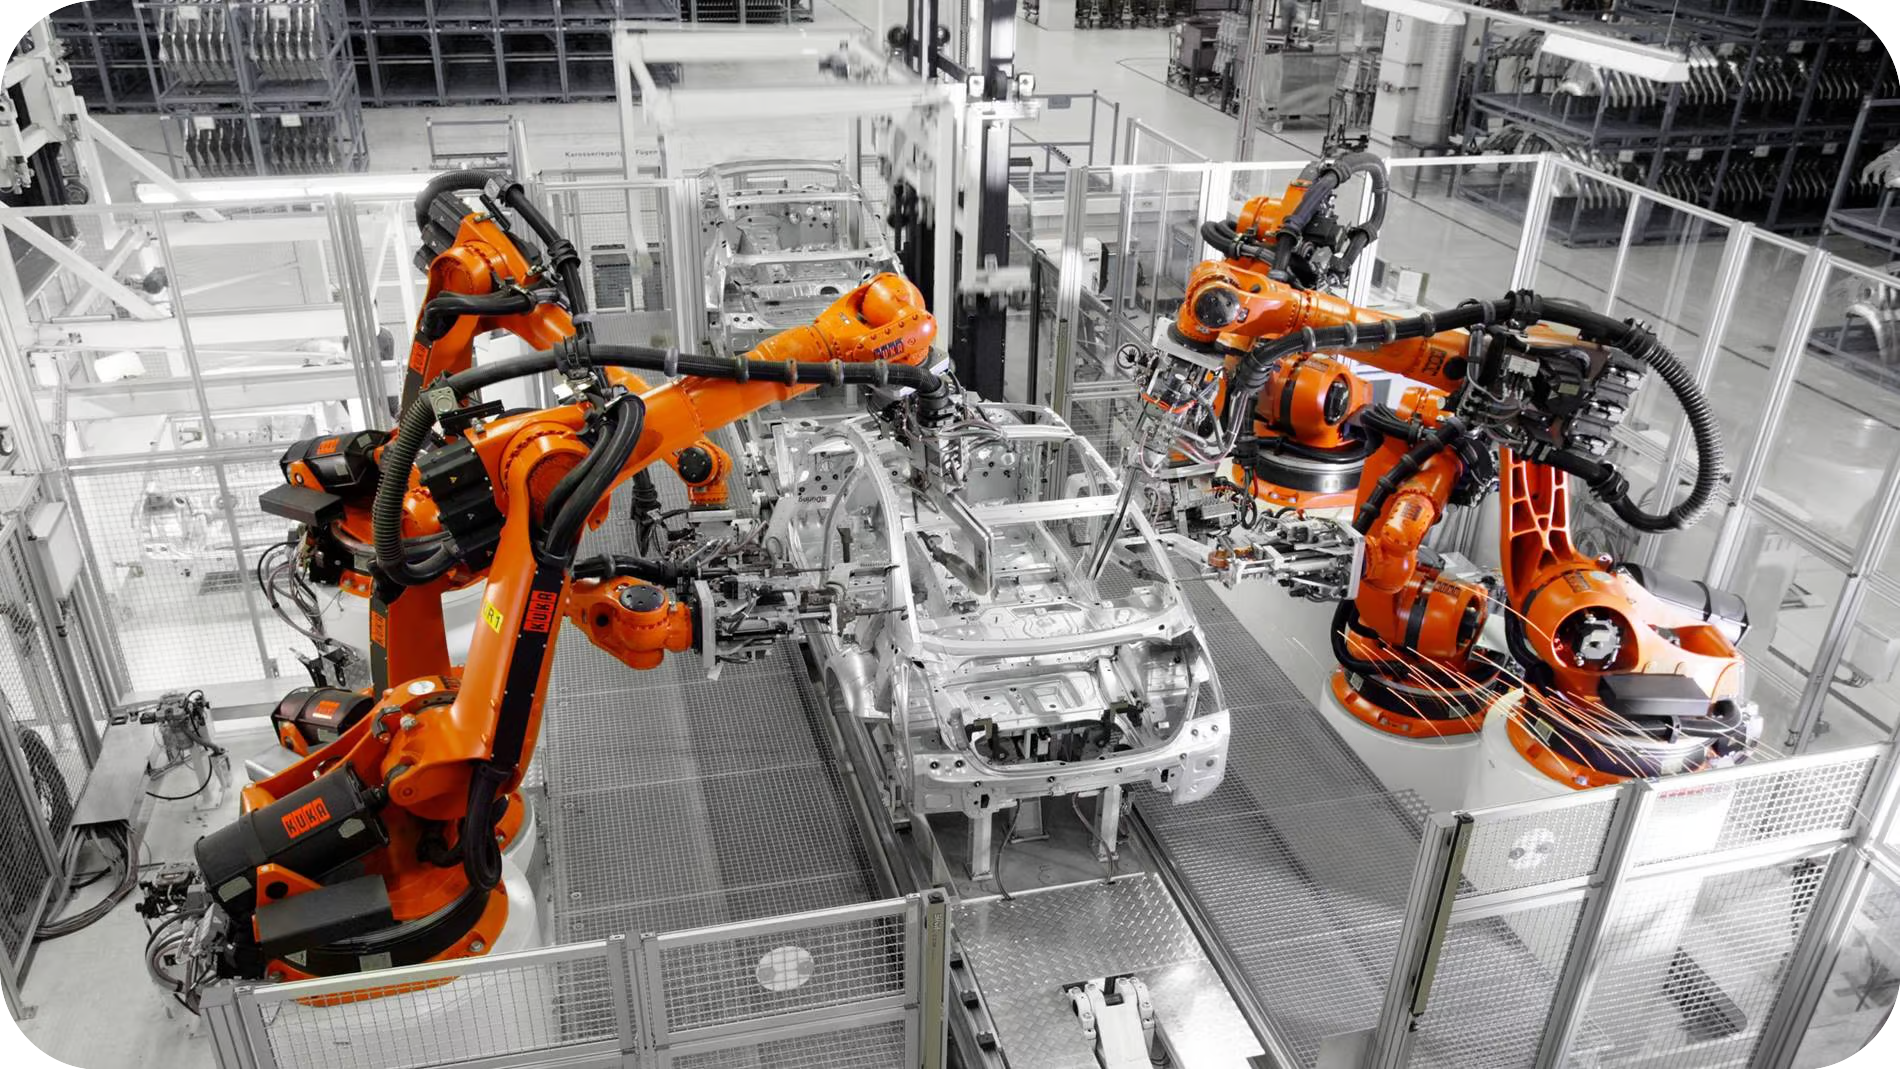
\includegraphics[width=0.9\textwidth]{src/introduction/img/industrial_robot.png}
    \caption{Industrial robot}
    \label{fig:industrial_robot}
  \end{subfigure}%
  \begin{subfigure}{0.5\textwidth}
    \centering
    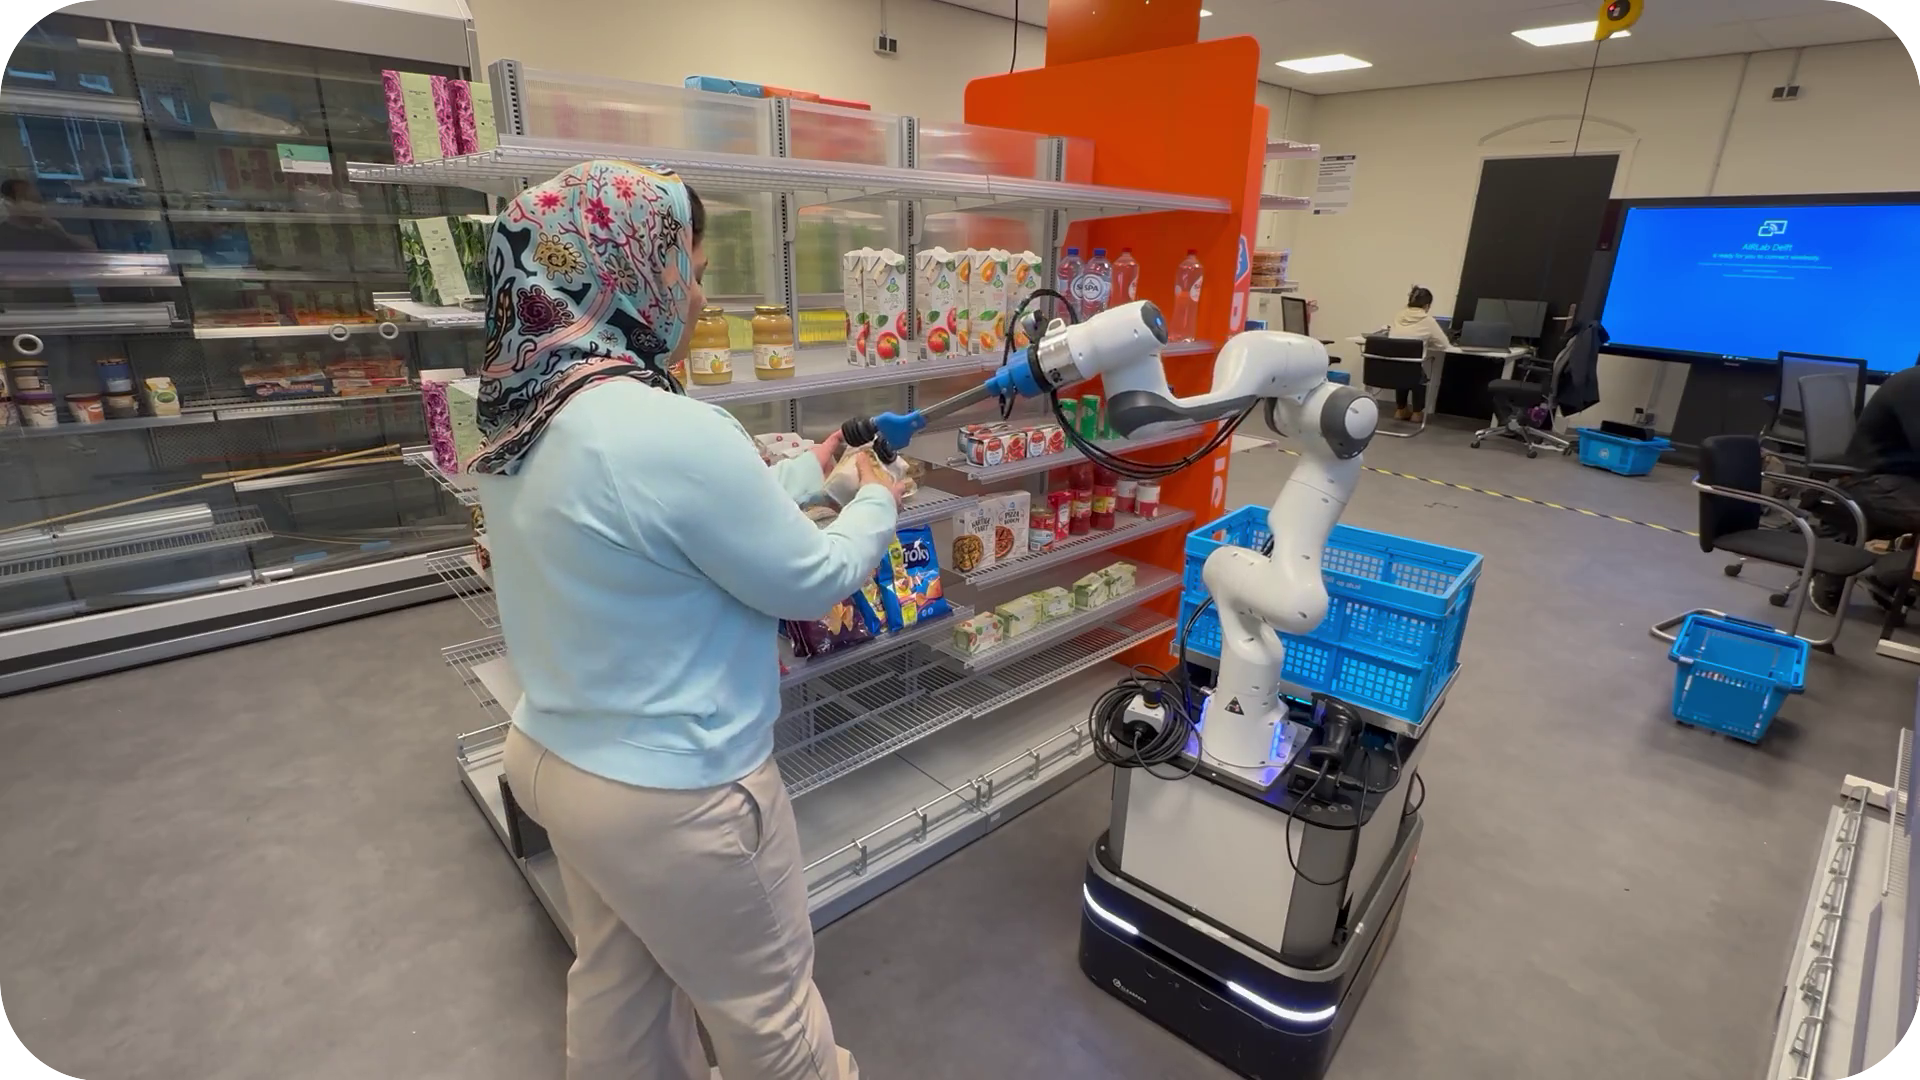
\includegraphics[width=0.9\textwidth]{src/introduction/img/collaborative_robot.png}
    \caption{Collaborative robot}
    \label{fig:collaborative_robot}
  \end{subfigure}
  \caption{The difference between environments where robots
  used to live in (left) and where we expect them to operate
  in the future (right).}
  \label{fig:different_robots}
\end{figure}

Next to
safety, robots must be equipped with a similar level of
mobility as humans to perform meaningful tasks. Mobility of
industrial robots is limited as they are statically
attached to structural elements. In that sense, they become
part of the building and exhibit no mobility. Placing
robots in environments, that are built with the mobility of
humans in mind, requires to unlock robots from the static
sockets.

In summary, helping an aging societies to deal with labor
shortage, the next generation of robots must be safe for
humans while equipped with the same mobility capabilities.

\subsection{Mobile manipulation}
\label{sec:mobile_manipulation}

One key feature of modern robots for human-shared
environments, is mobility. The combination of highly mobile
ground vehicles and manipulators is referred to as mobile
manipulation. This concept enables robots to navigate and
interact with their surroundings in ways previously deemed
challenging. By endowing robots with the ability to move and
manipulate objects in diverse environments, we further open
avenues for addressing the mentioned societal challenges.
Specifically, mobile manipulators could be used for tasks
from warehouse operations, restocking shelves, and package
delivery to intricate processes like food harvesting.
By placing robots onto moving bases, necessary mobility for
human-shared environment can be achieved.

\subsection{Challenges in robotics}

However, despite their potential, robots are noticeably
absent from human-shared environments. The complexities of
such spaces, coupled with safety constraints, present
formidable challenges. This is where \ac{tg}
becomes pivotal as one of the basic building blocks for
robotics software stacks. It determines the commands sent to
the motors in real-time, orchestrating a harmonious movement
that brings the robot closer to its goal while ensuring the
safety of itself and its environment.

While the hardware is ready for deployment, the
missing link lies in methods for generating trajectories
that prioritize safety while providing high success rates.
This dissertation embarks on a journey to unravel this
critical aspect of robotics, exploring innovative \ac{tg}
methods that not only unlock the potential of
robotic hardware but also lead to a world where robots
seamlessly coexist with humans in shared spaces.

\section{Limitations of current approaches}

In the quest for effective \ac{tg}, various
methods have been proposed, each with its set of advantages and
drawbacks.

The classical setup for robots --where they have
proven to be quite effective-- is behind fences. This setup
simplifies \ac{tg} dramatically as collision
avoidance can be done during the installation process and
trajectories can remain unchanged for the entire lifetime of
the robots. Therefore, high computational costs for
\ac{tg} are negligible as it is only performed
once during installation. However, their Achilles' heel lies
in their incapacity to adapt to dynamic, changing
environments.

Recognizing this limitation has spurred the rise of local
\ac{tg} methods, especially as robots are
expected to enter human-shared environments. However, even
within this domain, challenges persist. Pure control
approaches, exemplified by operational space control or
impedance control, offer speed and interpretability but fall
short in incorporating the entirety of the problem, such as
collision avoidance with itself and the environment or
joint limit avoidance.

With the aim for safe robots, many approaches these days are
founded on optimization problems, centered around an
objective function and constraints that favor safety
guarantees and optimality. Such approaches are often
referred to as model predictive control schemes or receding
horizon optimization \cite{hewing2020learning}. While
optimization-based methods have demonstrated success in
autonomous driving applications, they stumble when
confronted with real-time constraints in systems with
increased degrees of freedom due to high computational costs
\cite{spahn2021coupled}.

In the age of deep neural networks, learning-based
approaches have gained popularity as they promise similar
performance to optimization-based techniques. After all,
they solve the same problem, while changing the naming of
the objective function from cost function to loss (or
reward) function. Their major drawback lies in their
inability to integrate safety constraints in a principled
manner, often prone to overfitting specific use cases during
training and thus lacking generalizability when confronted
with new scenarios \cite{noroozi2023conventional}.
Computational costs are also often
mentioned when criticizing such approaches, but as
computational capacity increase rapidely, it seems little
justified. 

In the early days of robotics, potential field methods were
popular in the context of \ac{tg}.
They are based on the idea of modeling the robot as
a point in a potential field, where the goal is a minimum
and obstacles are maximac
~\cite{barraquand1992numerical,hwang1992potential}. This
approach is known to be computionally affordable and but
only covers the static components of the problem, and thus
ignores the dynamics of the robot.

Another notable contender from the same era is Cartesian
impedance control, praised for its rapid responsiveness and
perceived safety, \cite{hogan1985impedance}. Cartesian
impedance control models the point of interest on the
kinematic chain, usually the end-effector, as a
spring-damper-system attracted to the goal pose. In contrast
to potential field theory, the motion of the robot is thus
taken intro consideration. However, it falls short by not
encompassing crucial components for a collision-free
\ac{tg}. Modeling the point of interest of the robot as a
second-order differential equation raises the question
whether all components of the \ac{tg} problem can be handled
in this way. 

We can observe that modern approaches to \ac{tg} focus on the
practical side of \ac{tg} and often ignore the underlying
geometric structure \cite{Ratliff2015}. For example,
formulating the \ac{tg} problem in the Euclidean work space
of the end effector, as it is done 
in many optimization-based methods, is a simplification of 
the problem ignoring the configuration space of the robot.
Effectively, this approach uses a Euclidean geometry.
In contrast, the work space can also be modeled as a
Riemannian (or even non-Riemannian) manifold of the
configuration space. Then, other components, that live in 
different manifolds of the configuration space, can be
seemlessly integrated into the \ac{tg} problem \cite{Ratliff2015}.
This insight has lead to a series of different works
where \ac{tg} has been addressed purely geometrically
\cite{Ratliff2015,Cheng2019,Cheng2020,Ratliff2020,Xie2020}.

\section{Geometries in trajectory generation}
\label{sec:geometries_in_trajectory_generation}

In this dissertation, we recall and extend a framework
that allows to iteratively design \ac{tg} via
summation of individual behaviors. Individual behaviors are
designed as differential equations of second order for which
stability properties are conserved during summation.
This concept, elegantly formalized as \ac{fabrics}, offers
a nuanced understanding of \ac{tg}.
Informally speaking, the composition shapes the
landscape on which the trajectory is then generated.
Formally speaking, we gradually introduce terms into the
non-Riemannian metric shaping a smooth manifold of the
configuration space. In this thesis, we provide an important
extension to dynamic environments and give several use-cases
for this method.

\section{Contributions}
\label{sec:contributions}

This disseretation centers around two approaches to
\ac{tg}: (a) \ac{mpc} which formulates
\ac{tg} as an optimization problem which is
solved in a receding horizon fashion and (b) \ac{fabrics}
where \ac{tg} is formulated as a 
purely geometric problem.

This dissertation presents contributions to both methods in
the context of mobile manipulation and demonstrate the
usability with several robots and in a concrete application.
Specifically, we can list the following contributions:


\subsection{Advancements in \ac{mpc} for mobile manipulation}
\begin{enumerate}
    \item Enable real-time capable \ac{mpc} formulations for
      coupled \ac{tg} in mobile manipulators
      using \ac{fsd}.
    \item Conduct a quantitative comparison between \ac{mpc}
      formulations and \ac{fabrics} for various types of
      robots, providing insights into their relative
      strengths and limitations.
    \item In this work, a 3D collision avoidance for the
      entire kinematic chain is proposed that allows safe
      arm motion during all phases of the locomotion
      process. In contrast to the work of
      \cite{Avanzini2018}, no dynamic weighting is required,
      as collision avoidance can be guaranteed for the
      entire kinematic chain. The proposed work does not
      require an object detection method to allow safe
      motion, as the raw point cloud can be processed using
      free convex region generation \cite{Liu2017}.
      Moreover, our approach reduces overall operational
      time while introducing a convex region generation to
      keep the computational costs low. \MS{Shorten}
\end{enumerate}

\subsection{Theoretical advancements in \ac{fabrics}}
\begin{enumerate}
    \setcounter{enumi}{2}
    \item Generalize the framework of \ac{fabrics}
      for dynamic environments, integrating moving obstacles
      through time-parameterized manifolds and incorporating
      path following via time-parameterized goal
      definitions.
    \item Extend the framework of \ac{fabrics} to
      accommodate non-holonomic robots, enhancing the
      applicability of the framework for a broader range of
      robots.
\end{enumerate}

\subsection{Practical contributions of \ac{fabrics}}
\begin{enumerate}
    \setcounter{enumi}{4}
    \item Formulate \ac{fabrics} in a symbolic
      manner to enhance computational efficiency at runtime.
    \item Propose the use of Bayesian optimization for
      automated parameter tuning of \ac{fabrics},
      streamlining the optimization process and improving
      performance.
    \item Integrate implicit environment representations
      into \ac{fabrics}, reducing requirements on
      the perception pipeline and enhancing robustness in
      dynamic environments.
    \item Introduce learning-from-demonstration techniques
      for \ac{fabrics}, simplifying trajectory
      programming and improving usability.
\end{enumerate}

\subsection{Demonstration in a Real-world Setting:}
\begin{enumerate}
    \setcounter{enumi}{8}
    \item Demonstrate the usability of \ac{fabrics}
      in a prototype application, specifically in the
      context of order-picking in supermarkets, showcasing
      real-world applicability and effectiveness.
\end{enumerate}

These contributions collectively advance the field of mobile
manipulation and \ac{tg}, offering novel
solutions to address key challenges and paving the way for
future research and development efforts.





\section{Outline}

After this introduction, this dissertation first introduces
relevant literature in the field of \ac{tg}
and motion planning. Then, we summarize the required tools
from optimal control and from differential geometry to
understand the main chapters. In chapter 4, we explore a
model predictive control formulation for whole body control
with a mobile manipulator. We provide important steps to
handle the complexity of the problem. Then, we derive a
generalization of optimization fabrics to dynamic
environments, including contour tracking and avoidance with
moving obstacles. Chapter 6 highlights the benefits of
formulating \ac{tg} in a symbolic way to
improve real-time capabilities and allow for online
parameter tuning. To relax the requirement for the
perception pipeline, we layout several ways to integrate
implicit environment representations into the framework of
optimization fabrics in chapter 7. Finally, we conclude this
thesis by summarizing the findings, their potential impact
on deploying robots in human-shared environments, and giving some
recommendations for future works.

\begin{figure}
  \begin{center}
    \input{src/introduction/img/visual_outline.pdf_tex}
  \end{center}
  \caption{Outline of this thesis}
  \label{fig:outline}
\end{figure}

